\section{Обзор и анализ существующих алгоритмов консенсуса}

Алгоритмы консенсуса предназначены для обеспечения согласованности данных и
состояний между узлами распределённой системы в условиях сетевых задержек,
частичных отказов и отсутствия общего глобального состояния. Для системы
распределённых вычислений это особенно важно, поскольку ошибка в согласовании
приводит не только к расхождению журналов реплик, но и к потере задач,
повторному выполнению команд, некорректному назначению вычислительных ролей и
нарушению целостности результатов вычислений.

В рамках невизантийской модели отказов наибольшее практическое значение
получили алгоритмы семейства Paxos и алгоритм Raft. Оба подхода обеспечивают
согласованное принятие решений на основе кворума, однако различаются по
структуре протокола, организации управления кластером и удобству использования
в системах с реплицируемым состоянием.

\subsection{Алгоритм Paxos}

Алгоритм Paxos является одним из наиболее известных классических алгоритмов
достижения консенсуса в распределённых системах. Он был предложен Л.~Лэмпортом
в работе \enquote{The Part-Time Parliament} \cite{lamport98}, а затем изложен в
более прикладной форме в статье \enquote{Paxos Made Simple} \cite{lamport01}.

В классическом Paxos обычно выделяют три логические роли:

\begin{itemize}
    \item предлагающие узлы, формирующие предложения;
    \item принимающие узлы, голосующие за принятие предложений;
    \item узлы, фиксирующие итоговое выбранное значение.
\end{itemize}

На практике эти роли могут совмещаться в одном процессе, однако их разделение
удобно для описания логики алгоритма. Каждое предложение задаётся парой $(n,
v)$, где $n$ --- уникальный номер предложения, а $v$ --- предлагаемое значение.
Корректность алгоритма обеспечивается тем, что номера предложений упорядочены и
позволяют однозначно различать более ранние и более поздние попытки
согласования.

Классический Paxos состоит из двух фаз. На первой фазе предлагающий узел
отправляет кворуму принимающих узлов сообщение подготовки $Prepare(n)$ и
пытается получить от них обещание не принимать предложения с меньшими номерами.
На второй фазе, получив кворум ответов, он отправляет сообщение принятия
$Accept(n, v)$. Значение считается выбранным, когда его принял кворум
принимающих узлов \cite{lamport01}.

Ключевое свойство Paxos основано на пересечении кворумов: любые два кворума
имеют хотя бы один общий узел. Благодаря этому, если некоторое значение уже
было выбрано, информация о нём неизбежно будет учтена в последующих раундах, и
противоречащее значение не сможет быть выбрано позже. Именно это обеспечивает
безопасность алгоритма.

Обобщённая структура раунда Paxos приведена на рис.~\ref{fig:paxos}. Из схемы
видно, что в базовом варианте для согласования даже одного значения требуется
последовательное выполнение двух фаз с обменом сообщениями между узлами
кворума.

\begin{figure}
  \centering
  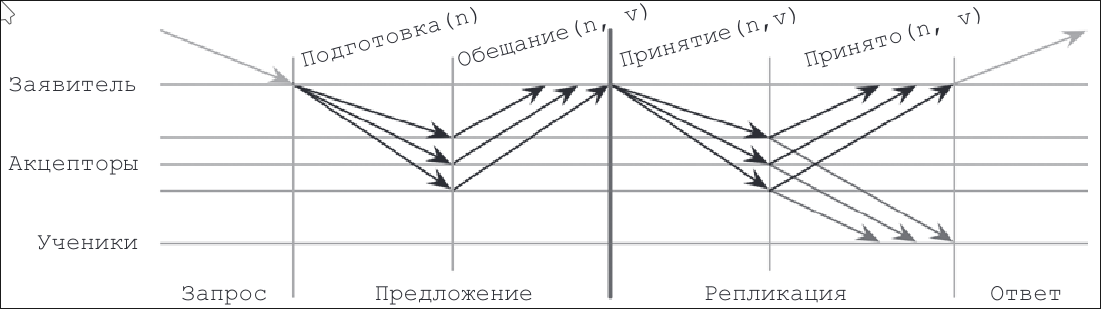
\includegraphics[scale=0.4]{inc/paxos.png}
  \caption{Структура раунда алгоритма Paxos}
  \label{fig:paxos}
\end{figure}

С точки зрения построения системы распределённых вычислений Paxos обладает
важным достоинством: он обеспечивает строгие гарантии согласованности даже в
условиях отказа части узлов. Однако его базовый вариант сложен в реализации по
нескольким причинам.

Во-первых, согласование каждого нового значения требует повторного выполнения
двух фаз протокола. Это увеличивает число сетевых обменов и создаёт
дополнительные задержки при последовательной обработке задач, что неудобно для
системы, в которой необходимо поддерживать общий журнал состояний, команд и
результатов.

Во-вторых, в классическом Paxos отсутствует явно выделенная и постоянно
действующая схема управления журналом. Алгоритм корректно решает задачу выбора
одного значения, однако переход от согласования отдельного значения к
согласованию последовательности операций требует дополнительных механизмов:
организации общего журнала, поддержания порядка записей, восстановления после
сбоев и согласования действий узлов при повторных раундах.

В-третьих, корректная реализация Paxos требует аккуратного обращения с номерами
предложений, кворумами и ранее принятыми значениями. Узел, инициирующий новый
раунд, обязан учитывать ответы принимающих узлов и, если некоторое значение уже
было принято ранее, продолжать именно его, а не произвольно предлагать новое.
Ошибка в этой логике приводит к нарушению безопасности, поэтому реализация
требует строгого соблюдения условий перехода между фазами и корректной
обработки устаревших, задержанных и повторно пришедших сообщений.

В-четвёртых, состояние принимающих узлов должно сохраняться таким образом,
чтобы после сбоя не терялись сведения о данных обещаниях и ранее принятых
предложениях. Иначе после перезапуска узел может начать вести себя так, как
будто часть истории согласования отсутствовала, что недопустимо для корректной
работы протокола.

Таким образом, сложность Paxos в реализации связана не столько с отдельными
шагами алгоритма, сколько с тем, что для построения полноценной системы
распределённых вычислений на его основе необходимо дополнительно решать задачи
управления журналом, выбора ведущего узла, сохранения устойчивого состояния и
корректной обработки конкурирующих раундов согласования.

\subsection{Алгоритм Multi-Paxos}

Для уменьшения накладных расходов классического Paxos используется его
расширение, обычно называемое многократным вариантом Paxos (Multi-Paxos). В
этом случае после стабилизации ведущего узла подготовительная фаза не
повторяется для каждой новой команды. Это позволяет использовать уже
достигнутое лидерство для последовательного согласования ряда записей журнала.

Для системы распределённых вычислений такое расширение существенно, поскольку
позволяет перейти от согласования отдельного значения к согласованию
последовательности операций: регистрации задачи, назначения исполнителя,
фиксации промежуточного состояния и записи итогового результата. Тем самым
многократный Paxos делает алгоритм более пригодным для построения
реплицируемого журнала.

Тем не менее даже в таком виде алгоритм сохраняет высокую концептуальную и
инженерную сложность. Хотя многократный вариант Paxos устраняет необходимость
повторять подготовительную фазу для каждой записи, его корректная реализация
всё равно требует поддерживать устойчивое состояние принимающих узлов,
обрабатывать смену ведущего узла, учитывать возможное пересечение и конкуренцию
раундов, а также обеспечивать непротиворечивое восстановление журнала после
сбоев.

Кроме того, многократный Paxos обычно описывается не как один жёстко
фиксированный протокол, а как семейство близких практических схем, в которых
разработчику необходимо самостоятельно принимать решения о порядке
восстановления, обработке пропусков в журнале, моменте фиксации записей и
взаимодействии с клиентскими запросами. Поэтому многократный Paxos является
эффективным, но сравнительно сложным средством построения отказоустойчивой
распределённой системы.

\subsection{Алгоритм Raft}

Алгоритм Raft был предложен Д.~Онгаро и Дж.~Устерхаутом как более понятная и
практически ориентированная альтернатива Paxos \cite{ongario14}. Его основная
идея заключается в явной декомпозиции задачи консенсуса на выбор лидера,
репликацию журнала и обеспечение свойств безопасности.

В Raft каждый узел находится в одном из трёх состояний:

\begin{itemize}
    \item последователь (follower);
    \item кандидат (candidate);
    \item лидер (leader).
\end{itemize}

При запуске узлы находятся в состоянии последователя. Если последователь в
течение тайм-аута выборов не получает сообщений от действующего лидера, он
увеличивает номер терма (term), переходит в состояние кандидата и рассылает запросы
голосования другим узлам. Если кандидат получает голоса большинства, он
становится лидером текущего терма \cite{ongario14}.

После избрания лидер начинает отправлять последователям регулярные служебные
сообщения, подтверждающие его активность. Эти сообщения одновременно могут
использоваться для репликации новых записей журнала. Каждая запись журнала
имеет индекс и номер терма. Для добавления записей лидер передаёт последователю
номер текущего терма, индекс и терм предыдущей записи, а также одну или
несколько новых записей. Последователь принимает новые записи только в том
случае, если его журнал согласуется с указанной предыдущей записью. При
обнаружении расхождения лидер повторяет попытку с более ранней позицией
журнала.

Запись считается зафиксированной, когда она сохранена на большинстве узлов.
После этого лидер может считать её согласованной и применять соответствующую
команду к состоянию системы. Существенно, что новым лидером может стать только
узел с достаточно актуальным журналом, поэтому зафиксированные записи не
теряются при смене лидера.

Обобщённая структура раунда Raft приведена на рис.~\ref{fig:raft}. По сравнению
с Paxos здесь явно выделены выборы лидера, поддержание лидерства и репликация
журнала, что делает алгоритм естественным для систем, где требуется единый
журнал состояний и команд.

\begin{figure}
  \centering
  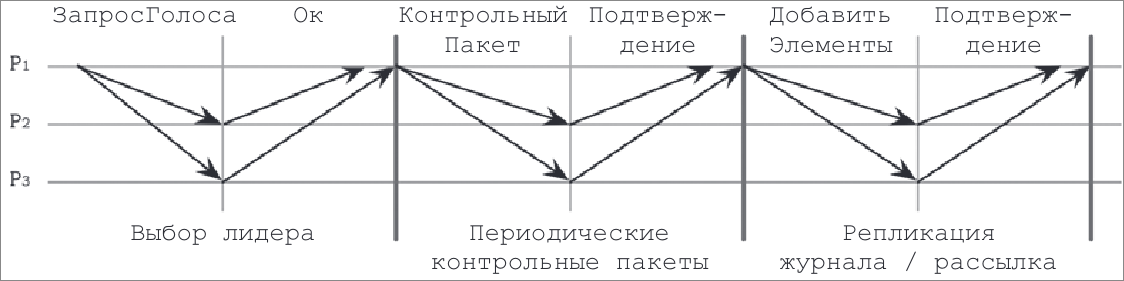
\includegraphics[scale=0.4]{inc/raft.png}
  \caption{Структура раунда алгоритма Raft}
  \label{fig:raft}
\end{figure}

Для системы распределённых вычислений Raft имеет ряд существенных достоинств.
Во-первых, он изначально ориентирован на ведение реплицируемого журнала, в
который естественным образом отображаются события жизненного цикла
вычислительной задачи. Во-вторых, наличие единственного лидера упрощает
координацию кластера: через лидера удобно проводить регистрацию задач, выдачу
команд рабочим узлам, фиксацию результатов и управление восстановлением после
сбоев. В-третьих, правила репликации и фиксации записей в Raft выражены явно,
что упрощает реализацию и сопровождение системы.

\subsection{Сравнительный анализ}

Алгоритмы Paxos и Raft обеспечивают консенсус в распределённой системе с
невизантийскими отказами и опираются на идею кворума. Оба алгоритма допускают
отказ части узлов и сохраняют безопасность даже при наличии сетевых задержек и
временной недоступности отдельных процессов. Следовательно, оба подхода в
принципе могут использоваться как основа отказоустойчивой системы
распределённых вычислений.

Однако их пригодность для такой системы различается. В Paxos первичной единицей
согласования является отдельное значение, а переход к последовательной
репликации множества значений требует дополнительных расширений. В Raft
реплицируемый журнал является центральной частью алгоритма с самого начала. Для
распределённой системы вычислений это особенно важно, поскольку её состояние
обычно представляется именно в виде последовательности согласованных операций
над журналом: приём задачи, изменение её статуса, назначение исполнителя,
подтверждение завершения, фиксация результата.

Существенно различается и организация управления кластером. В классическом
Paxos ведущий узел не является обязательной частью базовой модели, тогда как в
Raft лидер выступает центральным координатором. Для распределённой системы
вычислений это даёт практическое преимущество: упрощается маршрутизация
запросов, централизуется принятие решений о фиксации записей, а поведение
кластера становится более предсказуемым при сбоях и восстановлении узлов.

С инженерной точки зрения важным различием является и то, что в Paxos механизм
репликации журнала получается как развитие базовой схемы согласования, тогда
как в Raft он встроен в алгоритм изначально. По этой причине при реализации
Paxos разработчику приходится отдельно увязывать кворумное согласование
значений с ведением журнала, выбором ведущего узла, восстановлением после
отказов и обработкой конкурирующих раундов. В Raft эти элементы описаны как
части единого протокола, что делает поведение системы более прямолинейным и
предсказуемым.

Сравнение Paxos и Raft по основным техническим критериям приведено в
табл.~\ref{tab:paxos-raft-comparison}.

\begin{longtable}{|p{0.28\textwidth}|p{0.31\textwidth}|p{0.31\textwidth}|}
    \caption{Сравнение алгоритмов Paxos и Raft}
    \label{tab:paxos-raft-comparison} \\ \hline
    \textbf{Критерий} & \textbf{Paxos} & \textbf{Raft} \\ \hline
    \endfirsthead

    \caption*{Продолжение таблицы \ref{tab:paxos-raft-comparison}} \\ \hline
    \textbf{Критерий} & \textbf{Paxos} & \textbf{Raft} \\ \hline
    \endhead

    \hline
    \endfoot

    \hline
    \endlastfoot

    Базовая единица согласования &
    Одно значение; для последовательности значений обычно требуется Multi-Paxos &
    Запись реплицируемого журнала \\ \hline

    Организация управления &
    Лидер вводится в практических расширениях &
    Лидер является центральным элементом алгоритма \\ \hline

    Структура раунда &
    Две фазы: подготовка и принятие &
    Выборы лидера, подтверждение лидерства, репликация и фиксация записей \\ \hline

    Работа с журналом состояния &
    Журнал не является центральным элементом базовой модели; требуется дополнительная логика его ведения и восстановления &
    Журнал является основой алгоритма и репликации состояния \\ \hline

    Координация кластера &
    Требует доп.\ соглашений в практических реализациях &
    Естественно строится вокруг лидера \\ \hline

    Поведение при смене ведущего узла &
    Корректно, но логика сохранения значения задаётся через кворумы, номера предложений и устойчивое состояние узлов &
    Корректно, за счёт явных правил актуальности журнала и выборов лидера \\ \hline

    Удобство реализации системы распределённых вычислений &
    Требует дополнительного связывания кворумного согласования с ведением журнала, выбором ведущего узла и восстановлением после сбоев &
    Более естественно подходит для координации задач, репликации состояния и восстановления после сбоев \\ \hline

\end{longtable}

Итак, Paxos и его вариация представляют собой фундаментальную
основу невизантийского консенсуса и обеспечивают строгие гарантии
согласованности. Однако для системы распределённых вычислений особенно важны
удобство ведения реплицируемого журнала, простота координации узлов,
предсказуемость поведения при отказах и ясность структуры протокола. По этим
критериям алгоритм Raft лучше соответствует требованиям распределённой
вычислительной системы, хотя окончательное обоснование его выбора будет
приведено в конструкторской части работы.
